%\VignetteIndexEntry{pairheatmap Overview}
%\VignetteDepends{pairheatmap}
%\VignetteKeywords{pairheatmap}
%\VignetteKeywords{pairheatmap}
%\VignetteKeywords{pairheatmap}
%\VignettePackage{pairheatmap}
\documentclass[a4paper]{article}

\newcommand{\Rfunction}[1]{{\texttt{#1}}}
\newcommand{\Robject}[1]{{\texttt{#1}}}
\newcommand{\Rpackage}[1]{{\textit{#1}}}
\newcommand{\Rclass}[1]{{\textit{#1}}}
\newcommand{\Rmethod}[1]{{\textit{#1}}}

\author{Xiaoyong Sun$^\dagger$\footnote{johnsunx1@gmail.com}}

\usepackage{Sweave}
\begin{document}

\setkeys{Gin}{width=1\textwidth}

\title{Quick Guide for pairheatmap Package}
\maketitle
\begin{center}$^\dagger$McDermott Center for Human Growth \& Development \\ The University of Texas Southwestern Medical Center \\ Dallas, TX 75390, USA
\end{center}

\tableofcontents
%%%%%%%%%%%%%%%%%%%%%%%%%%%%%%%%%%%%%%%%%%%%%%

\section{Introduction}
Heatmap, as a visualization tool for data matrix, has been widely utilized in data analysis. pairheatmap is an R package to compare two heatmaps and discover links and patterns within and across groups. In the context of biology, group can be defined based on gene ontology or selected gene lists.
\section{Parameters}
\begin{figure}[h!tb]
\centering
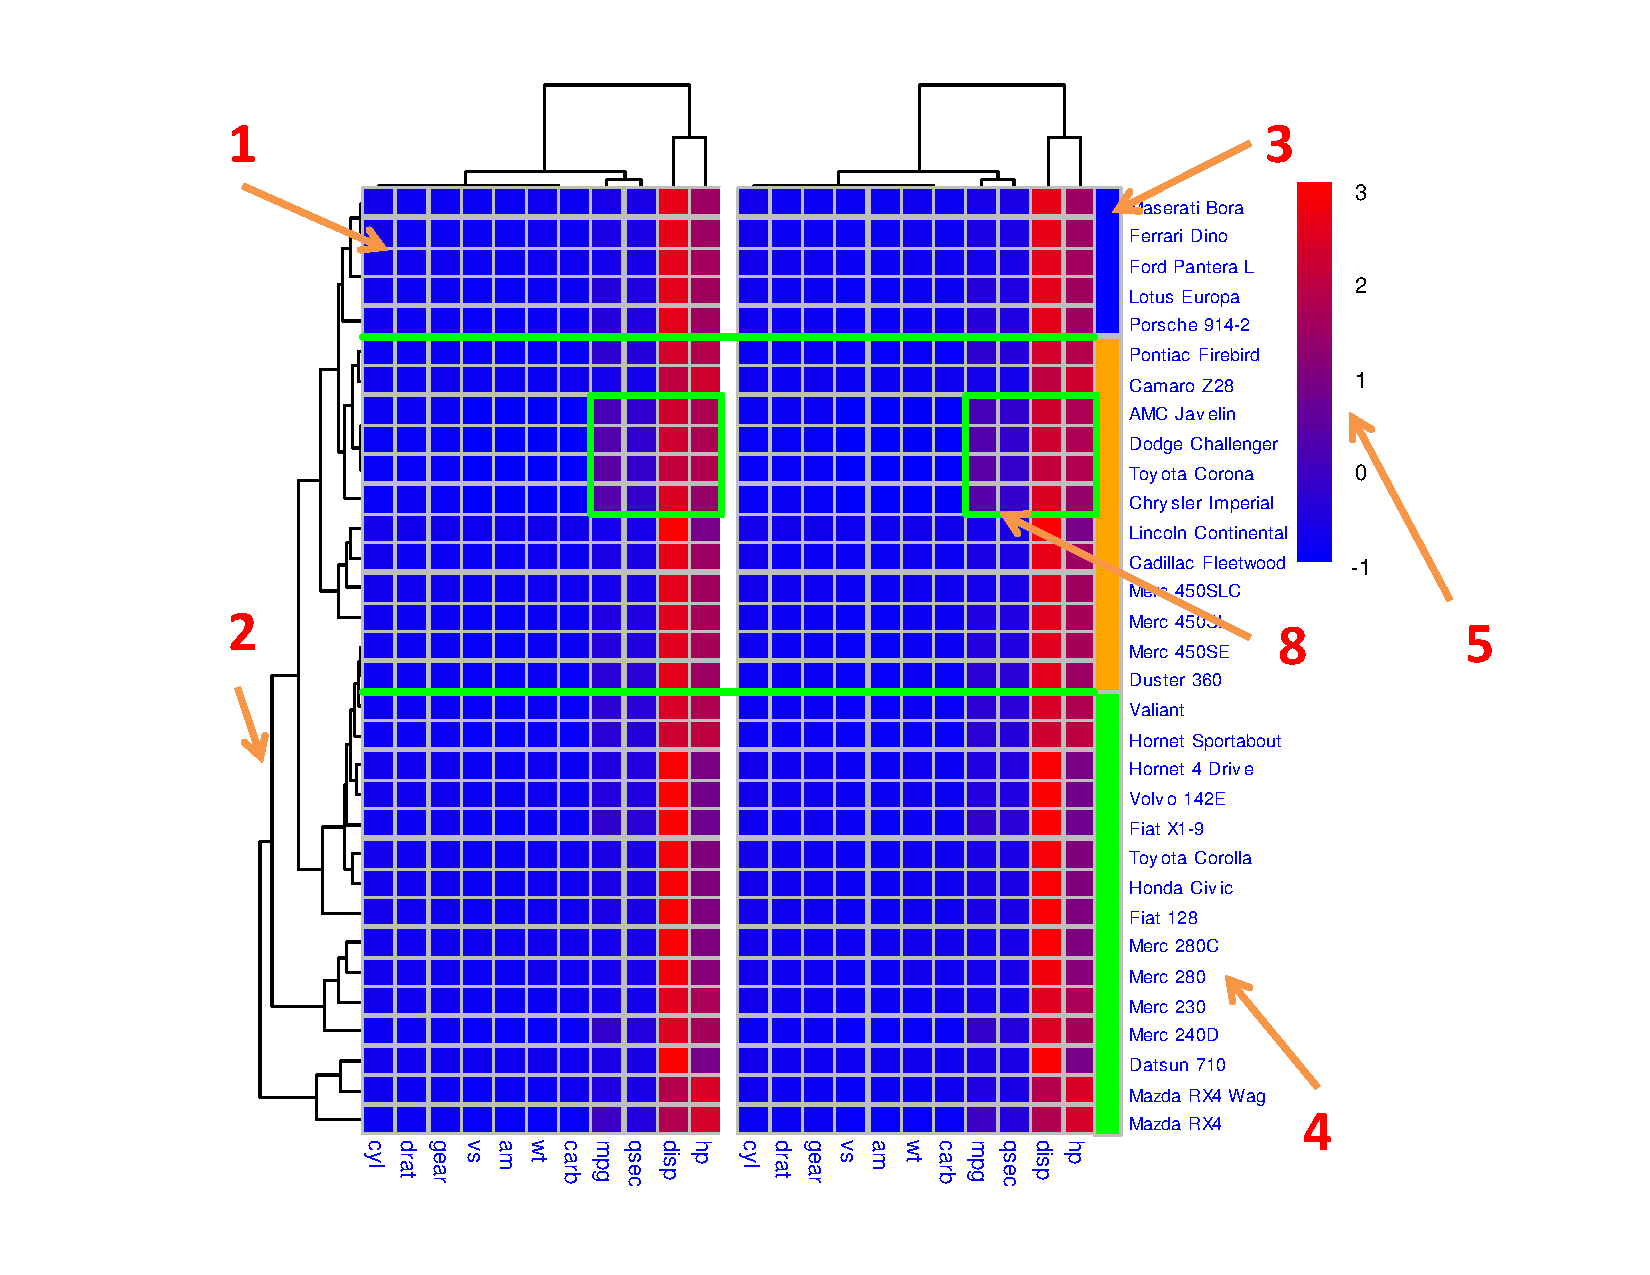
\includegraphics[scale=0.6]{figure.pdf}
\caption{Heatmaps marked with section numbers. 1: Data matrix; 2: Dendrogram; 3: Row group bar; 4: Row/Col names; 5: Legend; 8: Selected group.}
\label{figure}
\end{figure}
The main function for this package is \textit{pairheatmap}. There are many parameters for this function, including
\subsection{Data matrix}
\begin{itemize}
	\item data1: numeric matrix 1. It is considered as the standard matrix. 
	\item data2: numeric matrix 2. Its row order is same as that in data1. Its column order is either same as that in data1 or generated based on separate cluster method.	
	\item scale: character. It takes four values: "row", "col", "rowsep", "none". It indicates whether or not the data matrix is scaled together or separately in row/column direction. 
	\item matDist: the separate distance between two data matrices. Its value is the percent of the column width of the data matrix. If its value is 1, the distance between two matrices is exactly one data column.
	\item matrixBorderCol: the color of the data matrix border.
	\item colorStyle: the color style for the matrix cell. It takes four values: ``s1", ``s2", ``s3", ``s4". s1 ranges from blue to red; s2 ranges from green to red; s3 uses a default color style from R package, pheatmap; s4 ranges from white to black. 
\end{itemize}
\subsubsection{Examples}
\begin{verbatim}
pairheatmap(mtcars, mtcars[,1:5], scale="row")
pairheatmap(mtcars, mtcars[,1:5], scale="rowsep")
pairheatmap(mtcars, mtcars[,1:5], scale="col")
pairheatmap(mtcars, mtcars, colorStyle="s1")
pairheatmap(mtcars, mtcars, matDist=0.7)
\end{verbatim}
\subsection{Dendrogram}
\begin{itemize}
    \item dendrogram: character. It takes three values: ``row", ``col", ``both". It indicates whether or not to draw the row/col/both dendrogram(s). Methods and some codes are from R package: pheatmap.
\end{itemize}
\subsection{Row group bar}
Two matrices must have same number of row, and they may have different number of columns. So in pairheatmap, only row has been provided with group bar and group options. If you do need to look at columns, you can use ``\textit{t(data)}'' to get transpose of data matrix.\begin{itemize}
	\item rowGroupColor: logical value. It takes two values: ``TRUE", "FALSE". It indicates whether or not to draw the row group bar.
	\item rowGroupColor.choice: character. It works when rowGroupColor is set as TRUE. The character length must match the unique groups in the rowGroup. If it is not specified, the colorStyle is used as default value. 
\end{itemize}
\subsubsection{Examples}
\begin{verbatim}
pairheatmap(mtcars, mtcars,
     rowGroup=mtcars$gear,
     rowGroupColor=TRUE,
     rowGroupColor.choice = rev(c("blue", "orange", "green")))
\end{verbatim}
\subsection{Row/Col names}
\begin{itemize}
	\item rowNameColor: character string. It controls the label color of the row name.
	\item colNameColor: character string. It controls the label color of the column name.
	\item rowNameFontSize: numeric scalar. It controls the font size of the row name.
	\item colNameFontSize: numeric scalar. It controls the font size of the column name.
	\item rowNameGroupColor: character variable. The character length must match the unique groups in the rowGroup. It controls the color of different groups of row names. 
\end{itemize}
\subsubsection{Examples}
\begin{verbatim}
pairheatmap(mtcars, mtcars,
     rowGroup=mtcars$gear,
     rowNameFontSize=6,
     colNameFontSize=6,
     rowNameGroupColor=rev(c("blue",  "green", "orange")),
     rowNameColor="blue")
\end{verbatim}
\subsection{Legend}
\begin{itemize}
	\item legend.pos: character. It takes three values: ``top'', ``middle'', ``bottom''. It controls the position of the legend.
	\item legend.percent: numeric. It takes value from 0 to 1. If its value is 1, the height of the legend will be equal to the height of the heatmap.
	\item legend.fontsize: numeric. It controls the font size of the legend labels.
\end{itemize}
\subsubsection{Examples}
\begin{verbatim}
pairheatmap(mtcars, mtcars,
     legend.pos="middle", legend.percent=0.6, 
     legend.fontsize=7)
\end{verbatim}
\subsection{Group options}
This package has group options as,\newline
\begin{itemize}
	\item rowGroup: Row group variable.
	\item orderRowGroup: variable. The default value is ``NULL''. It is the row levels that should be ordered.
	\item groupBorder: character. It takes two values: "line", "rect". It controls the shape of the group border.
	\item groupBorder.lwd: numeric. It controls the line width of the groupBorder.
	\item groupBorder.col: character. It controls the line color of the groupBorder.
\end{itemize}
\subsection{Cluster analysis}
\begin{itemize}
	\item clusterMethod: character. It takes the follow values: ``ward", ``single", ``complete", ``average", ``mcquitty", ``median" or ``centroid".
	\item clusterMembers: NULL or a vector. See function: ``hclust'' of the package ``stats'' for details.
	\item clusterRow: logical. It takes two values: ``TRUE", "FALSE". It indicates whether or not to cluster rows.
	\item clusterCol: logical. It takes two values: ``TRUE", "FALSE". It indicates whether or not to cluster columns.
	\item clusterColTogether: logical. It takes two values: ``TRUE", "FALSE" (Default value). It indicates whether or not the columns of data matrix 2 follows the same clustering order of that in data matrix 1. If the column number of data matrix 2 is different from that of data matrix 1, only the columns matching those of data matrix 1 are reordered.	
	\end{itemize}
\subsubsection{Examples}
\begin{verbatim}
pairheatmap(mtcars, mtcars, clusterMethod="ward", clusterRow=FALSE)
pairheatmap(mtcars,  cbind(mtcars, mtcars), clusterColTogether=TRUE)
\end{verbatim}
\subsection{Selected group}
\begin{itemize}
	\item groupBorder.selectList: a list. It controls which group to be selected. It includes four components, ``xgroup.start'', ``xgroup.end'', ``ygroup.start'' and ``ygroup.end''.  The selected groups will be drawn with the same graphical parameters as groupBorder.
\end{itemize}
\subsubsection{Examples}
\begin{verbatim}
pairheatmap(mtcars,  cbind(mtcars, mtcars),
     groupBorder.selectList=
      list(xgroup.start=c(2,7), xgroup.end=c(4,9),
           ygroup.start=c(3,30), ygroup.end=c(10,32)
           ))
\end{verbatim}






\end{document}




